\chapter{Métodos de Solução}
Entre os métodos mais utilizados para a resolução de problemas de programação linear destaca-se o método simplex  e o método de pontos interiores. 
Depois da apresentação do método simplex,outros métodos com diferentes abordagens foram propostos \cite{Todd}. Porém, dentre os métodos existentes apenas o método de pontos interiores é atualmente competitivo em relação ao método simplex \apud{Bixby}{Munari}. 
A principal diferença entre esses dois métodos é que o método simplex busca a solução ótima em um dos vértices da região viável, enquanto o método de pontos interiores percorre o interior da região viável definindo um caminho até a solução ótima \cite{MaculanPI}. Além disso, uma outra diferença é que o simplex exige muitas iterações com cálculos simples, enquanto no método de pontos interiores poucas iterações são exigidas, porém com cálculos mais elaborados.
Apesar das vantagens do método de pontos interiores em relação ao método estudado neste trabalho, o método simplex possui melhor desempenho na resolução de problemas de pequeno e médio porte em relação ao método de pontos interiores.

\section{Método Simplex}
O método simplex é um dos algoritmos mais conhecidos para a resolução de problemas de programação linear. Surgiu há mais de 60 anos atrás e foi proposto por George Dantzig.  

É um método iterativo, e sua ideia principal consiste no fato de que a cada iteração uma nova solução é encontrada, sempre melhor que a anterior até o ponto em que a solução ótima é obtida. Outra característica do método é o fato de ser matricial, ou seja, os dados a serem calculados são armazenados em matrizes.  

Com a utilização do método, foi percebido que a cada iteração eram requeridos muitos cálculos sobre valores que nem sempre importavam para a iteração seguinte, fato que do ponto de vista computacional tornaria o método ineficiente. Esse método é chamado de método simplex padrão ou tabular. A partir desse fato foi desenvolvido o método simplex revisado visando a resolução de problemas de programação linear computacionalmente.

\subsection{Princípio Básico do Método}
A idéia do método simplex consiste em resolver repetidas vezes um sistema de equações lineares, e assim obter uma sucessão de soluções até encontrar a solução ótima. Ou seja, é um processo onde nos movemos de uma solução viável para outra sempre melhor ou pelo menos não pior.

Um problema de programação linear é sempre constituído de uma função objetivo e várias restrições. Geometricamente, essas restrições resultam em uma forma geométrica, no espaço n-dimensional sendo n o número de variáveis no modelo. E cada vértice dessa forma geométrica é considerado como uma possível solução, retomando o exemplo apresentado na seção 2.2.
\begin{center}
	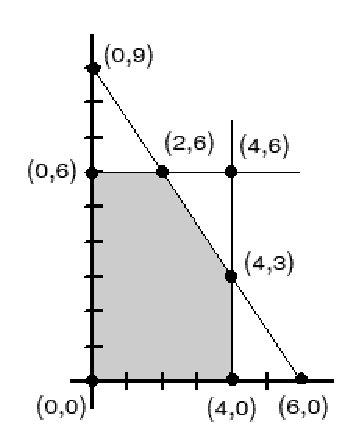
\includegraphics[scale=1.0]{graficos/graf_simplex_pontos}
	\captionof{figure}{Representação gráfica de um modelo de programação linear}
	\label{img:simplex_grafico_completo}
\end{center}

Nesse exemplo, de acordo com a representação geométrica do modelo, existem cinco possíveis soluções: ($x_{1}=0$ e $x_{2}=0$), ($x_{1}=0$ e $x_{2}=6$), ($x_{1}=2$ e $x_{2}=6$), ($x_{1}=4$ e $x_{2}=3$), ($x_{1}=4$ e $x_{2}=0$). Como o objetivo é maximizar, concluímos que a melhor solução é $x_{1}=2$ e  $x_{2}=6$, em que $z=36$. No método Simplex a cada iteração, antes da solução ótima ser obtida, é encontrada uma dessas possíveis soluções que se localizam nos vértices da forma geométrica.

\subsection{Descrição do Método Simplex Revisado}
O método simplex revisado surgiu como uma solução para evitar cálculos desnecessários. Esse método foi projetado para problemas a serem solucionados computacionalmente.

No simplex revisado, são armazenados na memória volátil apenas os dados realmente necessários. Além disso, os cálculos são realizados apenas sobre a coluna que é utilizada na iteração, o que evita cálculos com matrizes que poderiam acarretar uma imprecisão nos resultados.

Esse método mantém a característica do simplex, que é a troca entre a variável que entra na base e a que sai (as variáveis da base são as que contribuem para o valor da solução ótima), além de também exigir certo esforço computacional. Porém sua grande vantagem é a economia de tempo e espaço, que é garantida pelo modo como é desenvolvida a solução. 

Nesta seção são descritos os passos do algoritmo simplex revisado. O problema considerado é de maximização. A distinção entre matrizes, vetores e escalares foi feita da seguinte forma: letra maiúscula e negrito para matriz (\textbf{MATRIZ}); letra minúscula e negrito para vetor (\textbf{vetor}); letra em itálico para escalar (\textit{escalar}).

Considere o seguinte problema de programação linear:

$\\
Maximizar\ \mathbf{cx} \\
Sujeito\ a \\
\mathbf{Ax} \leq \mathbf{b} \\
\mathbf{x} \geq0$

O vetor $\mathbf{c}$, de coeficientes na função objetivo, é dividido em duas componentes: $\mathbf{c{_B}}$ e $\mathbf{c{_N}}$, coeficientes das variáveis básicas e não-básicas, respectivamente. Por analogia, o vetor $\mathbf{x}$, de incógnitas do problema, é subdividido em $\mathbf{x{_B}}$ e $\mathbf{x{_N}}$.  A matriz $\mathbf{A}$, de coeficientes das restrições, é dividida em duas submatrizes: $\mathbf{B}$ e $\mathbf{N}$, coeficientes das variáveis básicas e não-básicas, respectivamente. Os passos do algoritmo são os seguintes.\\

\begin{algorithm}[H]
\caption{Algoritmo do método Simplex Revisado}

Passo 1: Calcular o valor das variáveis básicas: \ \ $\mathbf{x_{b}}\ =\ \mathbf{B^{-1}b}\geq0$

Passo 2: Calcular o vetor multiplicador: \ \ $\mathbf{\lambda} \ =\ \mathbf{c{_B}B^{-1}}$

Passo 3: Escolher a variável que entra na base: $\mathbf{p}\ =\ \mathbf{c{_N}}-\mathbf{\lambda N}$

\uSe{Se \ \ $\mathbf{p}\ =\ (\mathbf{c{_N}}-\mathbf{\lambda N})\leq 0$} \ \ PARAR.

A solução \ \ $\mathbf{x{_B}}$ \ \ já é a solução ótima. 

Caso contrário, escolher uma coluna de $\mathbf{N}$, coluna $\mathbf{a{_k}}$, tal que $\mathit{p{_k}}\ =\ \mathit{c{_nk}}-\mathbf{\lambda a{_k}}> 0$

Um critério frequente é escolher a coluna $\mathbf{a{_k}}$ que resulte no maior valor de $\mathit{p{_k}}$.

Então, assumindo $\mathit{e} = \mathit{k}$, $\mathit{k}$ representa o índice da coluna, $\mathbf{a{_k}}$ representa a coluna de $\mathbf{A}$ candidata a entrar na base. 

Passo 4: Determinar a variável que sai da base. Para isso, calcula-se: $\mathbf{y}=\mathbf{B^{-1}a{_k}}$

Se \ \ $\forall i\mathit{\frac{b{_i}}{y{_i}}}\leq 0$ \ \ PARAR.

A solução é não-limitada. Caso contrário, calcular:\ \ 
$\forall i\ \underset{\underset{y{_i}>0}{1\leq i\leq m}}{Min}\begin{Bmatrix}
\mathit{\frac{b{_i}}{y{_i}}}
\end{Bmatrix}$ e guardar o índice correspondente a $s = i$. A variável $(x{_b}){_s}$ sai da base.

Passo 5: Criar a matriz $\mathbf{E}$.
$\mathbf{E}=(\mathbf{e{_1}},\mathbf{e{_2}},...,\mathbf{e{_s-1}},\mathbf{\gamma} , \mathbf{e{_s+1}},...,\mathbf{e{_m}})$

Onde, cada coluna da matriz é um vetor unitário com exceção da coluna $\mathit{s}$, que corresponde ao vetor $\mathbf{\gamma}$, calculado da seguinte maneira: \\
$\mathbf{\gamma^{t}}=\left( \mathit{\frac{-\alpha {_{1,e}}}{\alpha {_{s,e}}}}\ \mathit{\frac{-\alpha {_{2,e}}}{\alpha {_{s,e}}}}\ ...\ \mathit{\frac{-\alpha {_{s-1,e}}}{\alpha {_{s,e}}}}\ \mathit{\frac{1}{\alpha {_{s,e}}}\ \frac{-\alpha {_{s+1,e}}}{\alpha {_{s,e}}}}\ ...\ \mathit{\frac{-\alpha {_{m,e}}}{\alpha {_{s,e}}}} \right )$

Onde $\mathit{\alpha{_ie}}$ são os elementos vetor do $\mathbf{y}$.

Passo 6: Calcular nova matriz $\mathbf{B^{-1}}$: $\mathbf{B^{-1}} = \mathbf{EB^{-1}}$

Passo 7: Atualizar os vetores $\mathbf{c{_B}}$ e $\mathbf{x{_B}}$.
\end{algorithm}

\section{Método de Pontos Interiores}
Em 1984, Karmarkar revolucionou a área de programação linear com a publicação de um algoritmo de complexidade polinomial que apresentou bom desempenho quando aplicado a problemas práticos \cite{MaculanPI}. Essa publicação deu origem a um novo campo de pesquisa, chamado de método dos pontos interiores. 

O método de pontos interiores tem como principal característica realizar a busca por soluções no interior da região viável do problema, até encontrar a solução ótima \cite{Pinto}.
Em teoria, o método de pontos interiores é melhor que o método simplex, principalmente quando se leva em conta o critério de complexidade de pior caso. O método de pontos interiores possui complexidade polinomial, enquanto o método simplex possui complexidade exponencial No entanto, na prática ambos os métodos concorrem até hoje. Já que o sucesso do método depende da estrutura dos problemas, da esparsidade \footnote{Quando uma matriz possui uma grande proporção de elementos nulos diz-se que é uma matriz esparsa \cite{Munari}.} e da arquitetura dos computadores \cite{MaculanPI}.
